% Detaillierte Beschreibung bestimmter für das Programm wichtige Abläufe anhand von Sequenzdiagrammen. Es sollten etwa 3-4 charakteristische und interessante Abläufe ausgewählt werden.
\section{Crawler}

\subsection{Start des Crawlers}
Beim Starten des Crawlers werden sämtliche notwendigen Komponenten der Reihe nach gestartet. Dadurch wird garantiert, dass jede Komponente eine Umgebung vorfindet in der sie laufen kann und alle Ressourcen bereits zur Verfügung stehen. In \cref{fig:crawler_start} ist der Start des Crawlers beispielhaft mit 2 StatusProcessor's dargestellt.

\begin{figure}[htb]
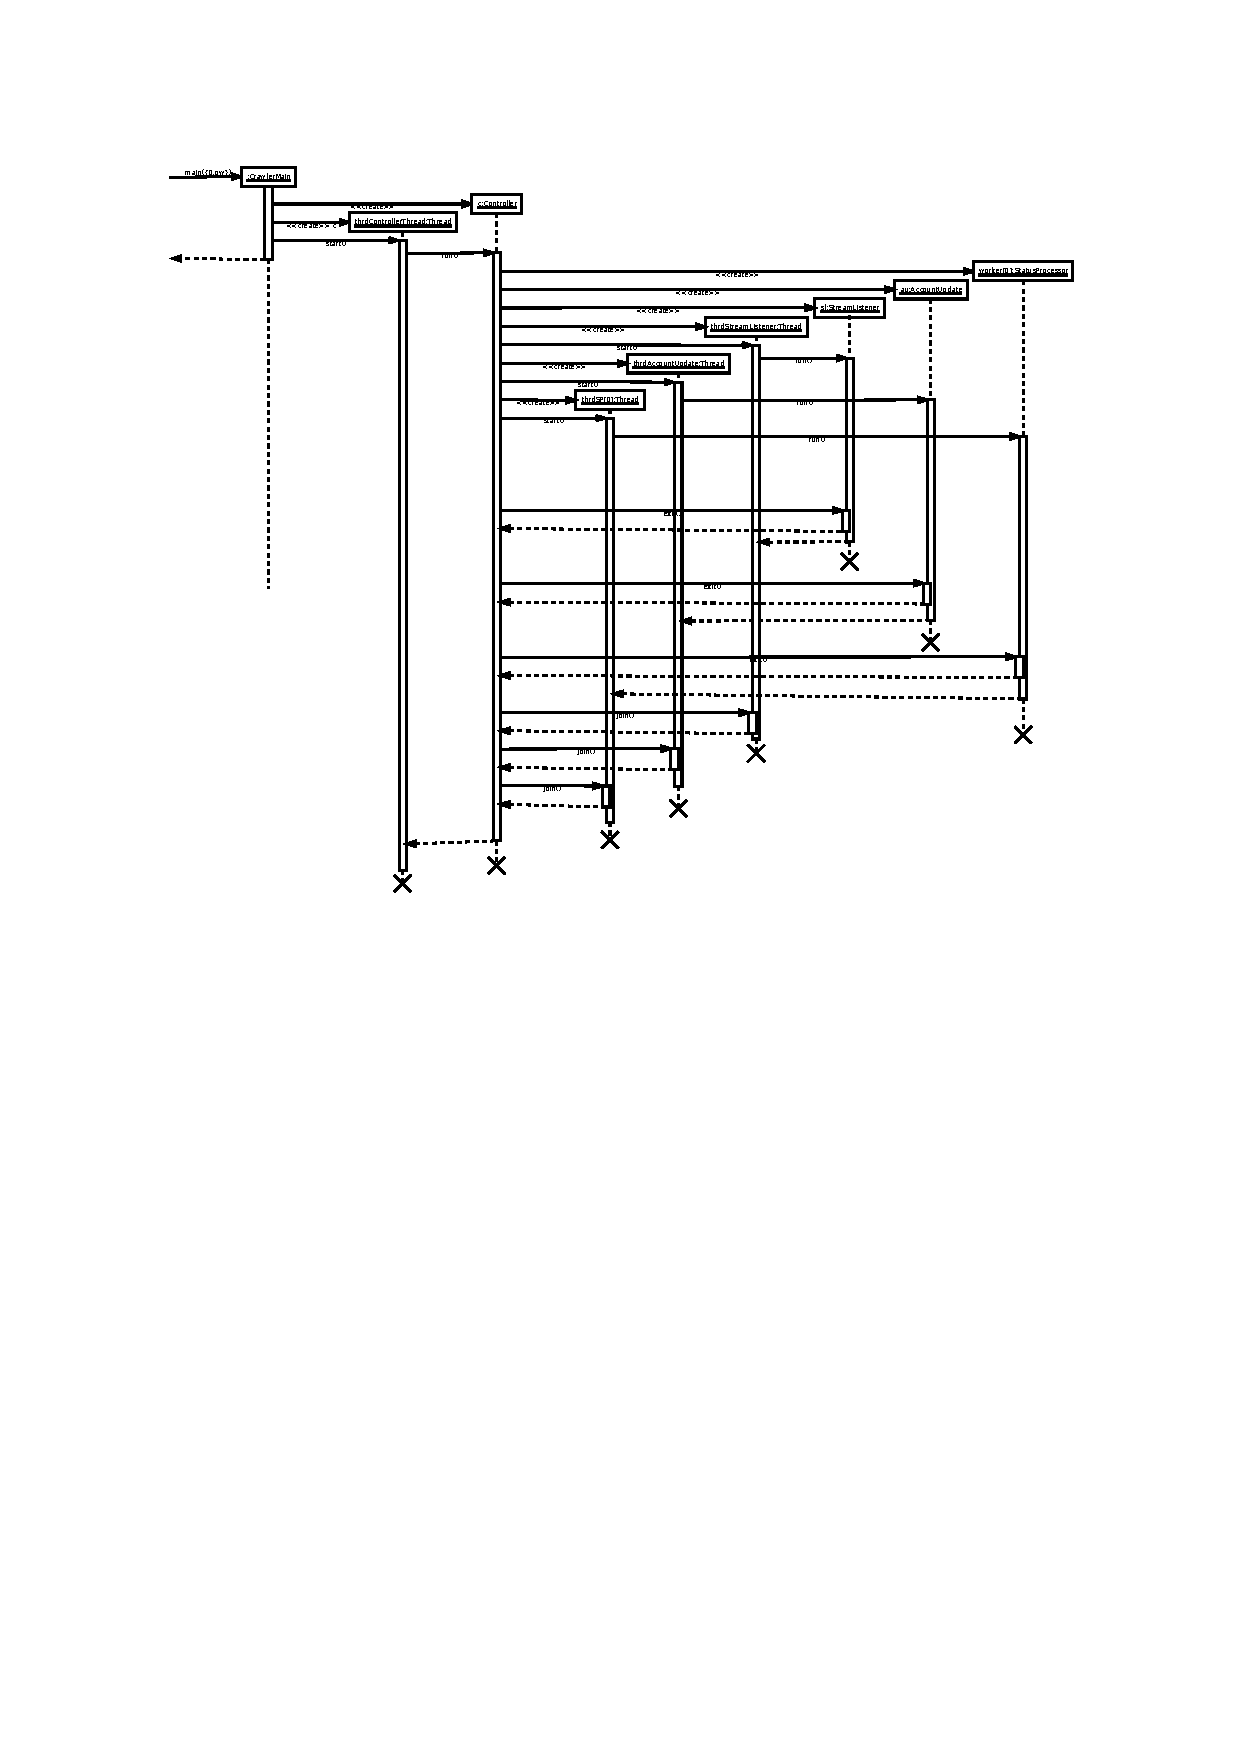
\includegraphics[width=\textwidth]{dia/crawler_start_sequence}
\caption{Sequenzdiagramm zum Start des Crawlers}
\label{fig:crawler_start}
\end{figure}

\subsection{Verarbeitung der Daten von Twitter}
Um zu verdeutlichen wie die Daten von Twitter innerhalb des Crawlers verarbeitet werden, ist in \cref{fig:crawler_process} der Datenfluss durch den Crawler exemplarisch dargestellt. Dabei werden die Daten von Twitter abgeholt, gepuffert, dann gefiltert und schlussendlich in die Datenbank geschrieben.

\begin{figure}[htb]
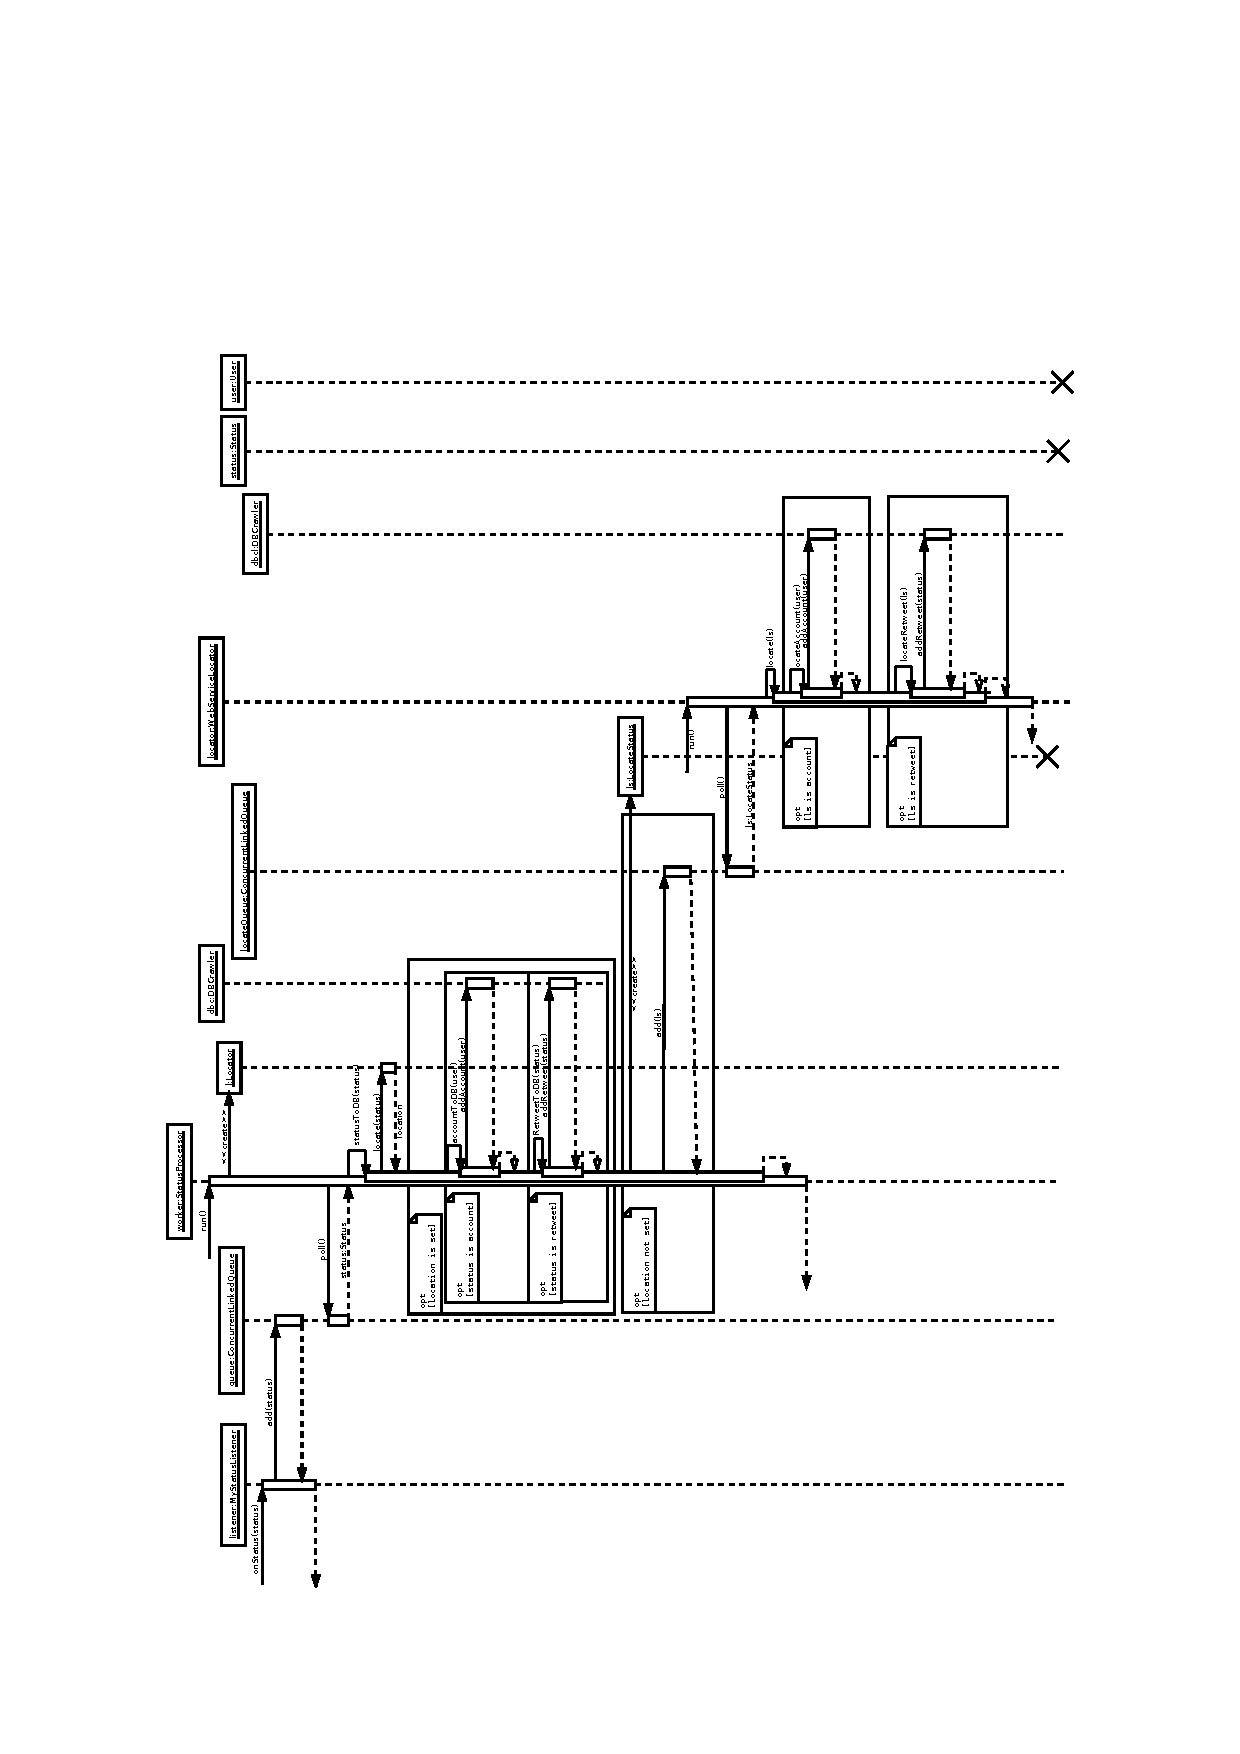
\includegraphics[width=\textwidth]{dia/crawler_process_sequence}
\caption{Sequenzdiagramm der Verarbeitung der Daten von Twitter}
\label{fig:crawler_process}
\end{figure}

\section{Kategorisierer}

\section{GUI}